\documentclass[12pt, a4paper, fleqn]{memoir}%makeidx

%******************************************************************************
% STYLE
%******************************************************************************
%******************************************************************************
% PACKAGES
%******************************************************************************
\usepackage{graphicx}
\usepackage{epsfig}
\usepackage{amsmath}
\usepackage{amssymb}
\usepackage{amsthm}
\usepackage{booktabs}
\usepackage{stmaryrd}
\usepackage{url}
\usepackage[figuresright]{rotating}
\usepackage{listings}
\usepackage{algorithm}
\usepackage{algpseudocode}
\usepackage{pifont}
\usepackage{ifsym}
\usepackage{relsize}
\usepackage[ansinew]{inputenc}
%\usepackage{dingbat}
\usepackage{hhline}
\usepackage{booktabs}
%\usepackage{xtab}
%\usepackage[margin=10pt,font={small,sf},labelfont=bf]{caption}
%\usepackage{tabularx}
%\usepackage{longtable}
%\usepackage{multirow}
\usepackage{color}
\usepackage{colortbl}
\usepackage{fancyvrb}
\usepackage{rotating}
\usepackage{makeidx}
\usepackage{MnSymbol}
\usepackage{textcomp}
%******************************************************************************
% INDEX GENERATION
%******************************************************************************
\makeindex

%******************************************************************************
% HYPEREF/ALGORITHM FIX
%******************************************************************************
\newcommand{\theHalgorithm}{\arabic{algorithm}}

% Konfiguration von hyperref
%\hypersetup{pdftex=true, colorlinks=true, breaklinks=true,
%   linkcolor=schwarz, menucolor=schwarz, pagecolor=schwarz, urlcolor=schwarz, citecolor=schwarz}

%******************************************************************************
% NUMBERING
%******************************************************************************
\numberwithin{algorithm}{chapter}
\numberwithin{figure}{chapter}

%******************************************************************************
% PAGE NUMBER IN BIBLIOGRAPHY
%******************************************************************************
\usepackage{citeref}
\renewcommand{\bibitempages}[1]{\newblock {\scriptsize [\mbox{cited at p.\ }#1]}}

%******************************************************************************
% PDF HYPERLINKS
%******************************************************************************
\ifpdf
  \pdfcompresslevel=9
        \usepackage[plainpages=false,pdfpagelabels,bookmarksnumbered,%
        colorlinks=true,%
        linkcolor=blue,%
        citecolor=blue,%
        filecolor=blue,%
        pagecolor=blue,%
        urlcolor=blue,%
        pdftex,
        unicode]{hyperref} 
    \input supp-mis.tex
    \input supp-pdf.tex
    \pdfimageresolution=600
    \usepackage{thumbpdf} 
\else
    \usepackage{hyperref}
\fi
\usepackage{memhfixc}

%******************************************************************************
% PAGE LAYOUT
%******************************************************************************
%\settypeblocksize{*}{32pc}{1.618}
%\setlrmargins{*}{1.47in}{*}
%\setulmargins{*}{*}{1.3}
%\setheadfoot{\onelineskip}{2\onelineskip}
%\setheaderspaces{*}{2\onelineskip}{*}
%\def\baselinestretch{1.1}
%\checkandfixthelayout



\newcolumntype{H}[1]{>{\columncolor[gray]{0.90}}p{#1}}
\newcolumntype{I}[1]{>{\centering\columncolor[gray]{0.90}}p{#1}}
\newcolumntype{q}[1]{>{\centering}p{#1}}
\renewcommand{\arraystretch}{1.25}
%******************************************************************************
% CHAPTER AND SECTION STYLE
%******************************************************************************
\makechapterstyle{mychapterstyle}{%
    \renewcommand{\chapnamefont}{\LARGE\sffamily\bfseries}%
    \renewcommand{\chapnumfont}{\LARGE\sffamily\bfseries}%
    \renewcommand{\chaptitlefont}{\Huge\sffamily\bfseries}%
    \renewcommand{\printchaptertitle}[1]{%
        \chaptitlefont\hrule height 0.5pt \vspace{1em}%
        {##1}\vspace{1em}\hrule height 0.5pt%
        }%
    \renewcommand{\printchapternum}{%
        \chapnumfont\thechapter%
        }%
}
\chapterstyle{mychapterstyle}
\setsecheadstyle{\Large\sffamily\bfseries}
\setsubsecheadstyle{\large\sffamily\bfseries}
\setsubsubsecheadstyle{\normalfont\sffamily\bfseries}
\setparaheadstyle{\normalfont\sffamily}
\makeevenhead{headings}{\thepage}{}{\small\slshape\leftmark}
\makeoddhead{headings}{\small\slshape\rightmark}{}{\thepage}

%******************************************************************************
% TABLE OF CONTENTS STYLE
%******************************************************************************
\settocdepth{subsection}
\setsecnumdepth{subsection}
\maxsecnumdepth{subsection}
\settocdepth{subsection}
\maxtocdepth{subsection}

%******************************************************************************
% COMMANDS FOR EPIGRAPHS
%******************************************************************************
\setlength{\epigraphwidth}{0.57\textwidth}
\setlength{\epigraphrule}{0pt}
\setlength{\beforeepigraphskip}{1\baselineskip}
\setlength{\afterepigraphskip}{2\baselineskip}
\newcommand{\epitext}{\sffamily\itshape}
\newcommand{\epiauthor}{\sffamily\scshape ---~}
\newcommand{\epititle}{\sffamily\itshape}
\newcommand{\epidate}{\sffamily\scshape}
\newcommand{\episkip}{\medskip}
\newcommand{\myepigraph}[4]{%
	\epigraph{\epitext #1\episkip}{\epiauthor #2\\\epititle #3 \epidate(#4)}\noindent}


%******************************************************************************
% FOOTNOTE STYLE
%******************************************************************************
\renewcommand{\thefootnote}{\fnsymbol{footnote}}

%******************************************************************************
% COLORS
%******************************************************************************
\usepackage{color}
\definecolor{greenyellow}   {cmyk}{0.15, 0   , 0.69, 0   }
\definecolor{yellow}        {cmyk}{0   , 0   , 1   , 0   }
\definecolor{goldenrod}     {cmyk}{0   , 0.10, 0.84, 0   }
\definecolor{dandelion}     {cmyk}{0   , 0.29, 0.84, 0   }
\definecolor{apricot}       {cmyk}{0   , 0.32, 0.52, 0   }
\definecolor{peach}         {cmyk}{0   , 0.50, 0.70, 0   }
\definecolor{melon}         {cmyk}{0   , 0.46, 0.50, 0   }
\definecolor{yelloworange}  {cmyk}{0   , 0.42, 1   , 0   }
\definecolor{orange}        {cmyk}{0   , 0.61, 0.87, 0   }
\definecolor{burntorange}   {cmyk}{0   , 0.51, 1   , 0   }
\definecolor{bittersweet}   {cmyk}{0   , 0.75, 1   , 0.24}
\definecolor{redorange}     {cmyk}{0   , 0.77, 0.87, 0   }
\definecolor{mahogany}      {cmyk}{0   , 0.85, 0.87, 0.35}
\definecolor{maroon}        {cmyk}{0   , 0.87, 0.68, 0.32}
\definecolor{brickred}      {cmyk}{0   , 0.89, 0.94, 0.28}
\definecolor{red}           {cmyk}{0   , 1   , 1   , 0   }
\definecolor{orangered}     {cmyk}{0   , 1   , 0.50, 0   }
\definecolor{rubinered}     {cmyk}{0   , 1   , 0.13, 0   }
\definecolor{wildstrawberry}{cmyk}{0   , 0.96, 0.39, 0   }
\definecolor{salmon}        {cmyk}{0   , 0.53, 0.38, 0   }
\definecolor{carnationpink} {cmyk}{0   , 0.63, 0   , 0   }
\definecolor{magenta}       {cmyk}{0   , 1   , 0   , 0   }
\definecolor{violetred}     {cmyk}{0   , 0.81, 0   , 0   }
\definecolor{rhodamine}     {cmyk}{0   , 0.82, 0   , 0   }
\definecolor{mulberry}      {cmyk}{0.34, 0.90, 0   , 0.02}
\definecolor{redviolet}     {cmyk}{0.07, 0.90, 0   , 0.34}
\definecolor{fuchsia}       {cmyk}{0.47, 0.91, 0   , 0.08}
\definecolor{lavender}      {cmyk}{0   , 0.48, 0   , 0   }
\definecolor{thistle}       {cmyk}{0.12, 0.59, 0   , 0   }
\definecolor{orchid}        {cmyk}{0.32, 0.64, 0   , 0   }
\definecolor{darkorchid}    {cmyk}{0.40, 0.80, 0.20, 0   }
\definecolor{purple}        {cmyk}{0.45, 0.86, 0   , 0   }
\definecolor{plum}          {cmyk}{0.50, 1   , 0   , 0   }
\definecolor{violet}        {cmyk}{0.79, 0.88, 0   , 0   }
\definecolor{royalpurple}   {cmyk}{0.75, 0.90, 0   , 0   }
\definecolor{blueviolet}    {cmyk}{0.86, 0.91, 0   , 0.04}
\definecolor{periwinkle}    {cmyk}{0.57, 0.55, 0   , 0   }
\definecolor{cadetblue}     {cmyk}{0.62, 0.57, 0.23, 0   }
\definecolor{cornflowerblue}{cmyk}{0.65, 0.13, 0   , 0   }
\definecolor{midnightblue}  {cmyk}{0.98, 0.13, 0   , 0.43}
\definecolor{navyblue}      {cmyk}{0.94, 0.54, 0   , 0   }
\definecolor{royalblue}     {cmyk}{1   , 0.50, 0   , 0   }
\definecolor{blue}          {cmyk}{1   , 1   , 0   , 0   }
\definecolor{cerulean}      {cmyk}{0.94, 0.11, 0   , 0   }
\definecolor{cyan}          {cmyk}{1   , 0   , 0   , 0   }
\definecolor{processblue}   {cmyk}{0.96, 0   , 0   , 0   }
\definecolor{skyblue}       {cmyk}{0.62, 0   , 0.12, 0   }
\definecolor{turquoise}     {cmyk}{0.85, 0   , 0.20, 0   }
\definecolor{tealblue}      {cmyk}{0.86, 0   , 0.34, 0.02}
\definecolor{aquamarine}    {cmyk}{0.82, 0   , 0.30, 0   }
\definecolor{bluegreen}     {cmyk}{0.85, 0   , 0.33, 0   }
\definecolor{emerald}       {cmyk}{1   , 0   , 0.50, 0   }
\definecolor{junglegreen}   {cmyk}{0.99, 0   , 0.52, 0   }
\definecolor{seagreen}      {cmyk}{0.69, 0   , 0.50, 0   }
\definecolor{green}         {cmyk}{1   , 0   , 1   , 0   }
\definecolor{forestgreen}   {cmyk}{0.91, 0   , 0.88, 0.12}
\definecolor{pinegreen}     {cmyk}{0.92, 0   , 0.59, 0.25}
\definecolor{limegreen}     {cmyk}{0.50, 0   , 1   , 0   }
\definecolor{yellowgreen}   {cmyk}{0.44, 0   , 0.74, 0   }
\definecolor{springgreen}   {cmyk}{0.26, 0   , 0.76, 0   }
\definecolor{olivegreen}    {cmyk}{0.64, 0   , 0.95, 0.40}
\definecolor{rawsienna}     {cmyk}{0   , 0.72, 1   , 0.45}
\definecolor{sepia}         {cmyk}{0   , 0.83, 1   , 0.70}
\definecolor{brown}         {cmyk}{0   , 0.81, 1   , 0.60}
\definecolor{tan}           {cmyk}{0.14, 0.42, 0.56, 0   }
\definecolor{gray}          {cmyk}{0   , 0   , 0   , 0.50}
\definecolor{black}         {cmyk}{0   , 0   , 0   , 1   }
\definecolor{white}         {cmyk}{0   , 0   , 0   , 0   } 
\definecolor{cell}          {cmyk}{0   , 0   , 0   , 0.25} 
\definecolor{stahlblau}		  {rgb} {0.2,0.56,0.84}
\definecolor{graurot}       {rgb} {0.62,0.15,0.15}
\definecolor{schwarz}       {rgb} {0.0,0.0,0.0}


%******************************************************************************
% BEGIN DOCUMENT
%******************************************************************************
\begin{document}

%******************************************************************************
% FRONT MATTER
%******************************************************************************
\frontmatter

%******************************************************************************
% EMPTY PAGE
%******************************************************************************
\pagestyle{empty}
This is actually the first page of the thesis and will be discarded after the print out. This is done because 
the title page has to be an even page. The memoir style package used by this template makes different indentations 
for odd and even pages which is usally done for better readability.  
\clearpage
%******************************************************************************
% TITLE PAGE
%******************************************************************************
\pagestyle{empty}
\rmfamily
\noindent
\begin{center}
University of Augsburg\\
Faculty of Applied Computer Science\\
Department of Computer Science\\
Bachelor Program in Computer Science\\
\end{center}
\begin{figure}[h]
\centering

\includegraphics[width=0.25\textwidth]{logo.png}
\end{figure}
\vfill\vfill
\begin{center}
\Large
Bachelor Thesis\\
\end{center}
\vspace{2.0em}
\begin{center}
\Large
\LARGE Brief Title\\ \vspace{10pt} 
\Large Development of a Multi-User, Multi-Display application to increase Energy Awareness
\end{center}
\vspace{2.0em}
\begin{center}
    \normalsize
    submitted by\\
    \large
    Karim Aly\\
    \normalsize
    on 25.08.2013
\end{center}
\vspace{2.0em}
\begin{center}
    \normalsize
    Supervisor:\\ 
    Dipl.-Inf. Michael Wi�ner
\end{center}
%\begin{center}
%    \normalsize
%    Adviser:\\
%    Dipl.-Inf. Michael Wi�ner
%\end{center}
\begin{center}
    \normalsize
    Reviewers:\\
    Prof. Dr. Elisabeth Andr\'{e}\\
\end{center}
\cleardoublepage

%******************************************************************************
% DEDICATION
%******************************************************************************
\vspace*{\fill}
{\hfill\sffamily\itshape}This work is dedicated for my brothers who died in rabaa massacre.
\cleardoublepage

%******************************************************************************
% ABSTRACT
%******************************************************************************
\chapter*{Abstract}
%This is the place where the \textit{abstract} of your thesis is supposed to be. The abstract is an essential part of a thesis, providing a brief summary of the thesis. Students often do not recognise the importance of the abstract and thus do not spend the required time in order to produce a well defined abstract. You should realize that the abstract is the walking advertisement for your thesis. Any reader's interest in your work stands or falls with the motivation provided by your abstract. A student should know that usually the reviewer of his or her thesis start reading with the abstract and the summary while often just making quick scans over some parts of the main chapters. An abstract is what will and has to be remembered.
Energy is now a trending issue that the whole world is talking and is worried about , the energy consumption is increasing and the resources are limited so the world has to find other ways to produce energy and decrease the level of energy consumption by people and in order to solve such a problem, the problem has to be identified.
So by knowing this fact and using the new modern ways as pubic displays and multi-user applications which was proven to motivate people to interact with it regularly in a fun and innovative way and that's how the idea of creating a multi-user, multi-display application to motivate people to save more energy and let them know how much energy they use came. 
%******************************************************************************
% ACKNOWLEDGMENTS
%******************************************************************************
\chapter*{Acknowledgments}
I would like to thank Ahmed Mohamed for helping me in understanding some concepts in the pusher service also Gasser Akila and Youssef Madkour for their support.

%******************************************************************************
% STATEMENT & DECLARATION
%******************************************************************************
\chapter*{Statement and Declaration of Consent}
\vfill
\subsubsection*{\LARGE Statement}
Hereby I confirm that this thesis is my own work and that I have documented all sources used.
\vfill
\begin{flushleft}
Karim Aly
\end{flushleft}  
\begin{flushright}
Augsburg, 25.08.2013 
\end{flushright}
\vfill
\vfill
\subsubsection*{\LARGE Declaration of Consent}
Herewith I agree that my thesis will be made available through the library of the Computer Science Department.
\vfill
\begin{flushleft}
Karim Aly
\end{flushleft}  
\begin{flushright}
Augsburg, 25.08.2013
\end{flushright}
\vfill

%******************************************************************************
% TABLE OF CONTENTS
%******************************************************************************
\cleardoublepage
\rmfamily
\normalfont
\pagenumbering{roman}
\pagestyle{headings}
\tableofcontents


%******************************************************************************
% MAIN MATTER
%******************************************************************************
\mainmatter

%##########################################################
\chapter{Introduction}
\label{chap:Introduction}

\section{Motivation}
\label{sec:Motivation}
Energy is now one of the main concerns the world is worried about , energy resources are running out and people's energy consumption is increasing dramatically it was expected that from 2008 to 2030 world energy consumption is expected to increase more than 55\% (Refer here). Also energy consumption increase the rate of Carbon dioxide (CO2) in our environment which then leads to global warming and other environmental problems.
\\
\newline \noindent One of the comments that was online about this topic stated "It's weird how unaware we are as to how much energy we're really using" and this is very true people in their daily lives doesn't seem to know anything about their energy consumption , while cooking in the kitchen or even taking a shower or while working. So people needed anything which tells them their energy usage in a daily basis and also allow them to view and compare their energy usages to hope for a better energy usages.
\\
\newline \noindent Concerning public displays and multi-user applications many cities around the world now began to install public displays in many places like airports, stations, streets and many other locations since public displays have proven to motivate the users to interact with it and also help them in finding what they need in a fun and innovative way. For example the installation of interactive video wall in Copenhagen , the museum of Copenhagen decided to install a 12 meter mobile interactive video wall in the street which attracts 4000 visitors per day that talks about cultural geography and history of Copenhagen. Also the wall has a timeline toolbar which you can explore the city in different historical periods. Moreover visitors can add comments and photos and saving in on the screen and this content that the user generates can be browsed by other people as well, the wall also has a website in which users can input images from home or anyplace. In addition users can add their own photos using their mobile phones or USB.
\\
\newline \noindent Another example was in Singapore as part of Changi Millionaire campaign to further engage Singaporeans and visitors by an interactive augmented reality multimedia game at the Media Hub Wall at Orchard MRT Station. The users just stand in the specified place in front of the screen and see their images on the screen with flying virtual money in which they try to grab as much money as they could.
\\
\newline \noindent The reaction of users on both examples gave a very good impression about how users interact with public displays and how public displays applications could be the future generation of applications used in every place you go so that motivated 

\section{Objectives}
\label{sec:Objectives}

The aim of the project was first letting the people know how much energy they use on a daily basis because the first step to solve the problem is knowing where the problem is. To do that we decided to use modern ways like public displays and smart phones as explained in the previous section in order to motivate people and engage them better in the application. We wanted to create an application which will give every detail about user's energy consumption and how to improve it , also representing this data in a fun and a new way while keeping the competitive environment on as a motivation to save more energy.
\\
\newline \noindent Moreover, helping the user in saving energy in their daily lives by giving them tips about the things they usually do every day but they don't even know that it waste energy and giving them more efficient ways maybe this is one of the most important ways to change people attitude towards the energy consumption case. Of coarse this helps if not by decreasing the energy the user consume, but by letting the user know ways about how the energy can be wasted without him knowing so and instead of doing the task in lets say a x amount of energy, it ends up using double this amount.
\\
\newline \noindent The system had to be trusted,robust and user friendly so in order to try to achieve that, privacy profiles were implemented in order to give the user an option to hide his data if someone suddenly appears or even if he doesn't want anyone to check his consumption also to increase user trust and confidence in the application. Finally we wanted to take advantage of the multi-user setup to give the users an option to view charts together in order to compare their energy consumption with each other which we believe that will motivate them more to save energy.
%\section{Outline}
%\label{sec:Outline}

%##########################################################
\chapter{Related Work}
\label{chap:RelatedWork}

\section{Theoretical Background}
\label{sec:TheoreticalBackground}
%Figure \ref{fig:intro} shows an image while you can cite a paper with \cite{AmirPnueli1985} or several papers with \cite{ThomasRist2004, Rist2002}.
Many projects were done under this topic or related somehow to the use of public displays and multi-user applications also to the energy awareness topic.
\\
\newline \noindent The first paper was  a treasure hunt game which used Augmented reality technology and adaptive virtual gardens to design a game to motivate people to save energy the game consisted of 2 parts the first one was the Augmented reality quiz which is some questions related to the environment issues and there were clues at every station in the building which helped the user to go to the next one and answer the questions, this was done to increase people awareness about the energy issue. The second part was a dynamic visualisation which converted each team score to a status of a personal virtual garden so the users first start with a good health garden and according to the score they get the health of the garden differs if they keep on getting more points the health of the garden improve and this part was responsible for the motivation by using the gaming principles like prize and score and the factor that all the teams or users scores where available on the public display as the garden status.
\\
\newline \noindent The second project was about a system which helps create more smart solutions and apply it to energy devices like creating scheduled tasks for each individual device and also being able to track the number of users in a house hold and the energy consumption of each user device to save more energy, the project mainly focus on dealing with the problem that most of the energy monitoring devices only allow people to reduce their total energy without knowing exactly which devices consumed which amount of energy so its very hard using this systems to know how much each device or each individual is actually using.
\\
\newline \noindent So the system developed was named USEM (Ubiquitous Smart Energy Management) which aimed to assist users to save more energy without caring too much on knowing how would the system accomplish that. The system classified the devices into 2 categories which are regular devices and continuous devices. Regular devices were represented in devices which only take a set of time like TVs,washer and oven while continuous  devices were represented in devices that operate more automatically without interference from the user like air conditioners , refrigerators and water heaters. Also the system defined whats called by rules and tasks for regular devices and defined levels for continuous devices instead of rules and tasks. So the rule was about a set of conditions, once met the rule is executed while task is just a task which the user schedule the system to finish it. As for the level it is also about setting a set of conditions but for continuous devices and to be able to control and set all that from the USEM software user interface.
\\
\newline \noindent The third project was about the different interaction techniques that can be used to interact with personalized public displays in sensitive situations, mainly it compares 3 different interaction techniques which are direct,bodily and mobile-based. The project classified the whole process into three phases which are identification, navigation and collecting results. Also mentioned that using personalized public displays makes it easier for the user to extract his own data because it can be tailored to the user profile but on the other hand it may cause some privacy issues. The project simply explained the 3 main phases starting by the identification phase which is the logging in system and how the user logs in the system and his personal data is shown on the display then the navigation phase which is about the user being able to navigate through out the application to find the data he needs and finally the collecting results and logging-off phase which indicates that the user has found what he wants and whether or not the user wants to save it on his mobile then log off and the data is removed from the screen.
\\
\newline \noindent The project also discussed the 3 possible techniques when interacting with public displays which are direct,bodily and mobile-based, so lets take a glance at each of these techniques as discussed in the project. The direct interaction involves having an interactive tool to interact with the display which can be user's hand or NFC-enabled mobile phone , bodily interaction this technique is mainly about gestures and body postures and is usually supported by camera-based recognition and mobile-based technique which uses a mobile phone to control and interact with the public display. Each of them had their positive and negative sides also an experiment was made to test which interaction technique was preferred by the users in the 3 phases of interaction , the results were that users preferred mobile-based technique in Identification and Collecting results phase however users preferred direct technique in the navigation phase. Moreover it was recommended to have an auto-logout feature to increase security and trust in the system and using well known metaphors in interaction.
\\
\newline \noindent The fourth project was about how to protect and maintain user privacy on personalized public displays and the project investigates the possible profiles that can be created for the user to choose the best privacy option for him also it investigated how the relationship context affected user's choice in deciding his privacy profile. The project classified privacy protection to 5 groups ordered  by ascending protection level and they are: do noting, minimize, mask, remove private part, remove all. Experiment was made to test which of the 5 privacy levels the users preferred when a stranger,colleague and a friend suddenly appears on the display and the results were that generally no protection is needed when the person appeared is a friend , the users tend to choose a more powerful privacy profile when the person is an acquaintance and finally the users tend to choose the strongest protection privacy level when the person is a stranger.

%\begin{figure}[h]
%\centering
%\includegraphics[width=0.8\textwidth]{enten.jpg}
%\caption{The map of Entenhausen}
%\label{fig:intro}
%\end{figure}

%\section{Section}
%\label{sec:Section}

%\subsection{PseudoCode}
%\label{sec:PseudoCode}
%If you want to show the implementation of some algorithm that is essential to the solution found in your thesis then do not write plain prgoram code. Use an abstract pseudocode representation instead. No one wants to see \texttt{C++\texttrademark} code or \texttt{Java\texttrademark} code in your thesis because it is presumed that you are able so write such a program as a computer scientist. Generally, writing program code is bad style and just blows up your thesis but will never be read by anyone but you. It is nothing scientific but your handwork while your thesis should show that you are able to do research as a scientist. A pseudocode example could look like the following:
%\begin{algorithm}[h]
%\caption{The Dekker Algorithm}
%\label{algo:dekker}
%\begin{algorithmic}
%\Require $n \in \mathbb{N}$
%\Require $0 \leq i,turn \leq n$
%\Require $\forall 0 \leq j \leq n : (interrested[j] = false)$
%\Procedure{DekkerAlgorithm}{$n,i$}
%  \State $interrested[i] \leftarrow true$
%  \While {$\exists 0 \leq j \leq n : (j \neq i \wedge interrested[j] = true)$}
%  \If {$turn \neq i$}
%    \State $interrested[i] \leftarrow false$
%    \While {$turn \neq i$}
%    \EndWhile
%    \State $interrested[i] \leftarrow true$
%  \EndIf 
%  \EndWhile
%  \State $ $
%  \State $\text{\textbf{\color{red}CRITICAL SECTION}}$
%  \State $ $
%  \State $turn \leftarrow Random(n)$
%  \State $interrested[i] \leftarrow false$
%\EndProcedure
%\end{algorithmic}
	%\end{algorithm}

%Be sure that each pseudocode listing is listed in the list of algorithms at the end of your thesis.

%******************************************************************************
% CONCEPT AND IMPLEMENTATION
%******************************************************************************

\chapter{Concept And Implementation}
\label{chap:ConceptAndImplementation}

\section{Technologies Used}
\label{sec:TechnologiesUsed}
The technologies used in the project were Django framework that was used to handle the backend code which was represented in writing the server code and creating the models or the tables of the database in order to be able to store the information needed to run the application as for the connection between the display and the mobile, we faced a major problem at the beginning, since web sockets technology was agreed to be used and it wasn't supported by the android native mobile browsers another solution had to be found and that what led us to pusher. Pusher is a tool which helps the developers to create applications which involves realtime in it, also phone gap was used to help in writing HTML5 code and javascript to make native applications for multiple platforms so it helped in developing the backend of the mobile code which was simply javascript. For the front end code or the user interface which was represented in the design and the looks of the application, HTML5 and CSS3 were used to design the application user interface and twitter bootstrap was used also for the public display user interface with jquery to reach a more powerful design also Jquery mobile was used on the mobile side for both handling the user interface and the server side functionalities on the mobile, moreover charts were needed in the application so canvasjs chart engine was used in rendering the charts with the given data using HTML5 canvas to draw the required charts.

\section{Concept}
\label{sec:Concept}
So the concept was to create an application to help people to increase their energy awareness and help them to save more energy. Since the technology used was agreed to be HTML5 and Web sockets, the idea was to create a multi-user application in which each user can do actions in their specified space or slot on the screen and by using web sockets the connection were established between each user(mobile) and the display. Moreover charts is created for the user to check regularly to check their energy usage and they get to choose the duration they want to view their usage into.

%and the django framework was used as mentioned in the previous section to handle the backend code and to manage and create the models in the database in order to achieve such an application also canvasjs the javascript chart engine and pusher were used to draw user charts to illustrate their energy usage.

\section{Connection}
\label{sec:Connection}
\begin{figure}[H]
\centring
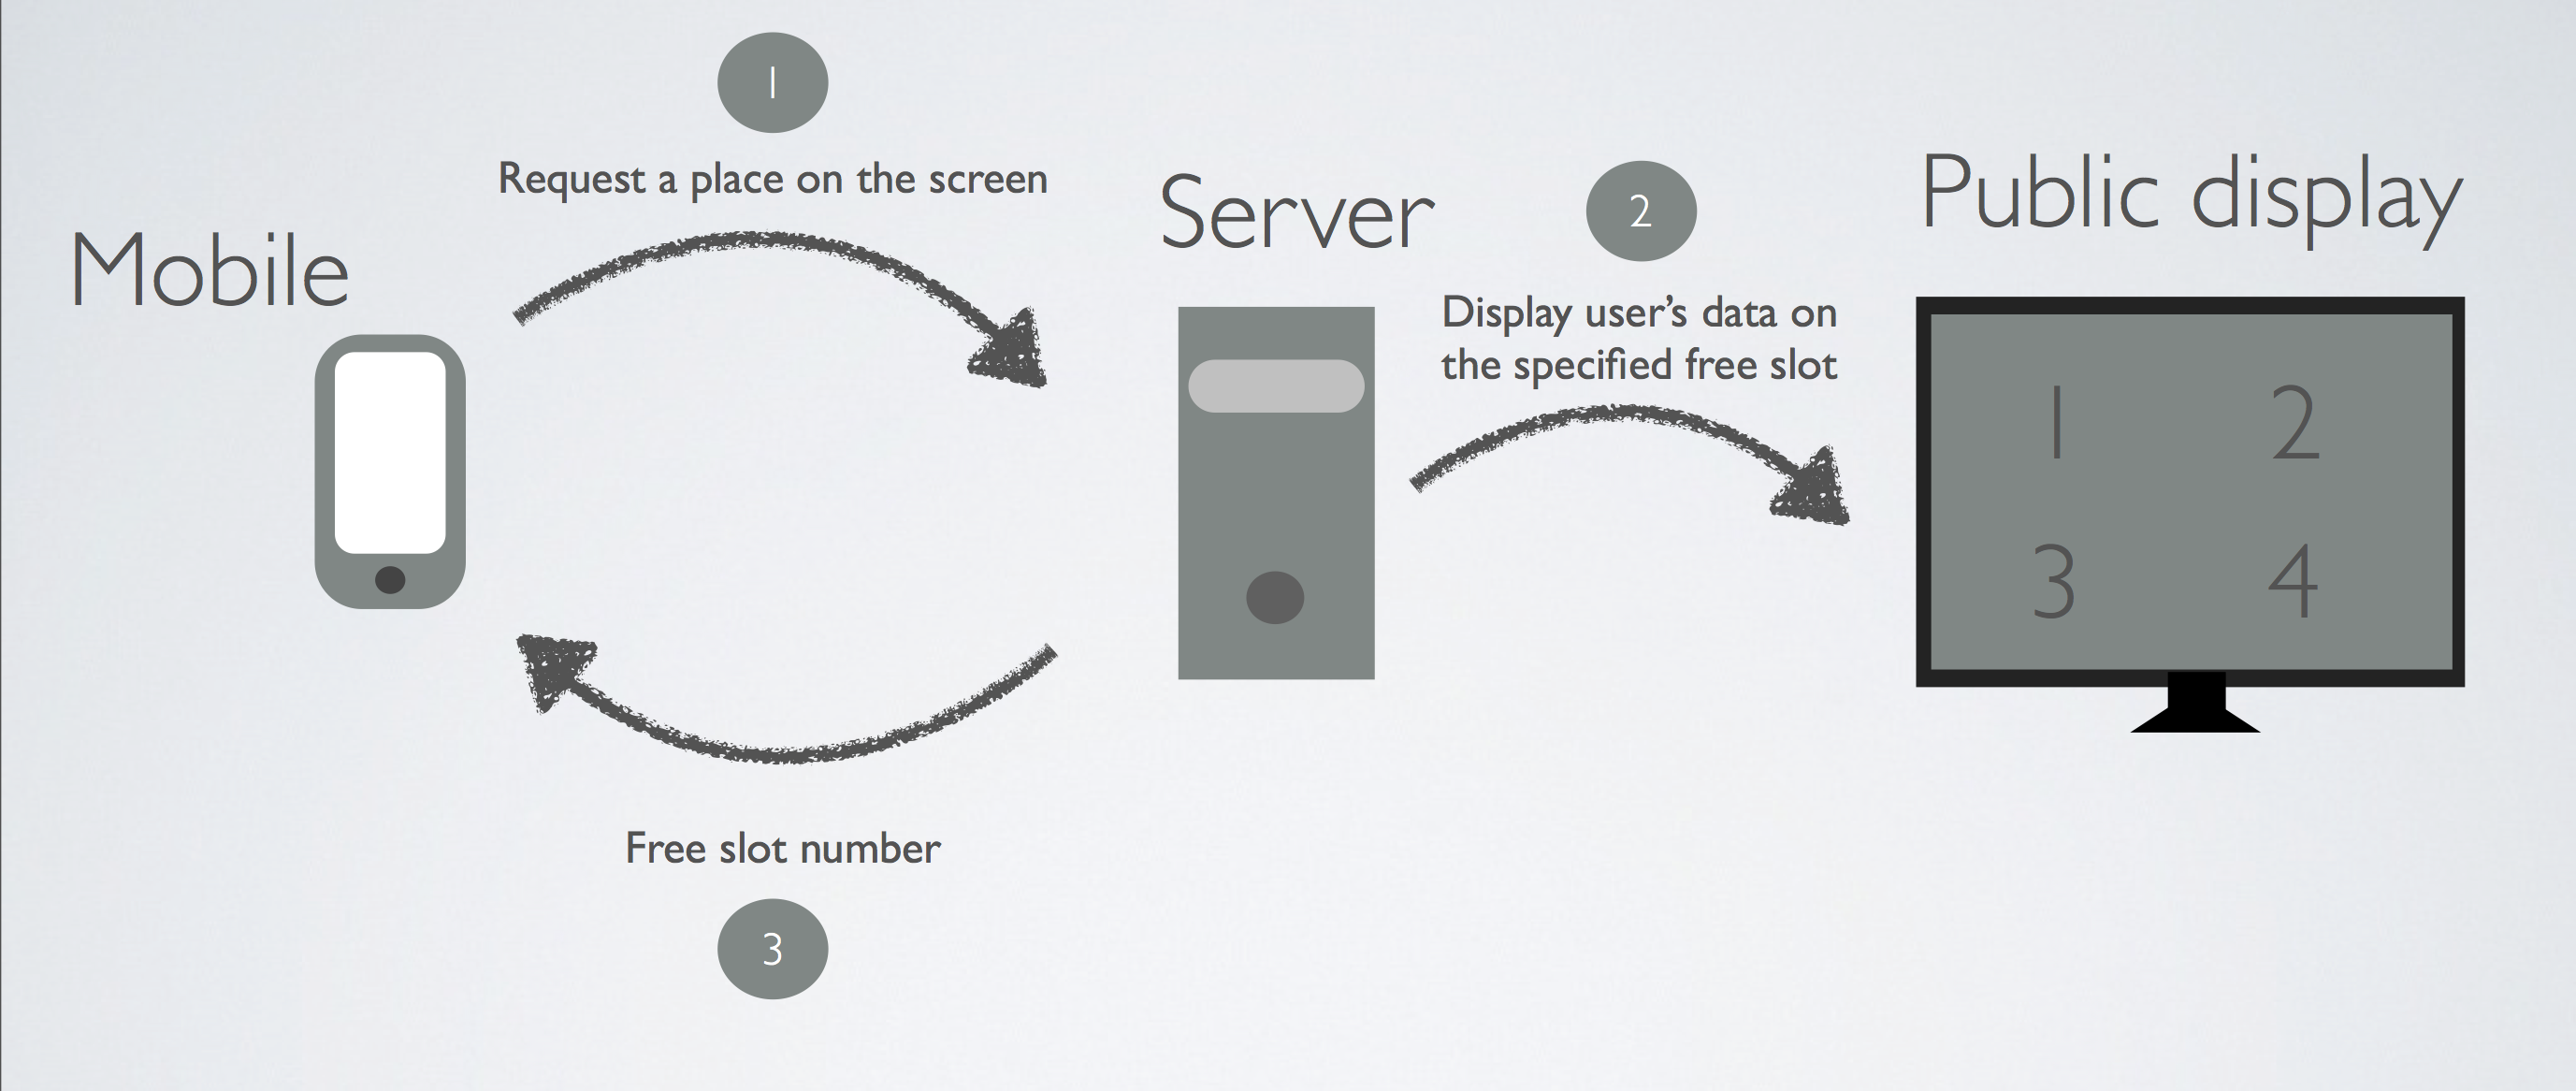
\includegraphics[width=1\textwidth]{Connection_figure.png}
\caption{This figure showing the connections made between the mobile,server and the display.}
\label{fig:Connection_figure}
\end{figure}
The connections in the project was mainly done using pusher first the user approaches the screen to find an introduction to the application and then the user has to click connect in order to start using the application.
Once the user presses connect on his mobile device a request is sent to the server which start executing the multi-user algorithm explained below in section \ref{sec:Multi-userSetup} after finding the specified free slot on the screen it saves the slot number and sends a signal to the public display to display the login page in the specified slot using a 4 channel connection system which consists of a channel for each slot of the screen , when the multi-user algorithm finds the free slot it connects to the channel that corresponds to this slot (will be explained briefly in section \ref{sec:Multi-userSetup}) avoiding clashing between users requests since each user on the display will have his own channel to send and receive requests and will also help in identifying each user actions and interactions with the system as you can see in Figure~\ref{fig:Connection_figure}.
\\
\newline \noindent As for the channels and the connections it can be seen in the following Figure~\ref{fig:ChannelsAndConnections}:

\begin{figure}[H]
\centring
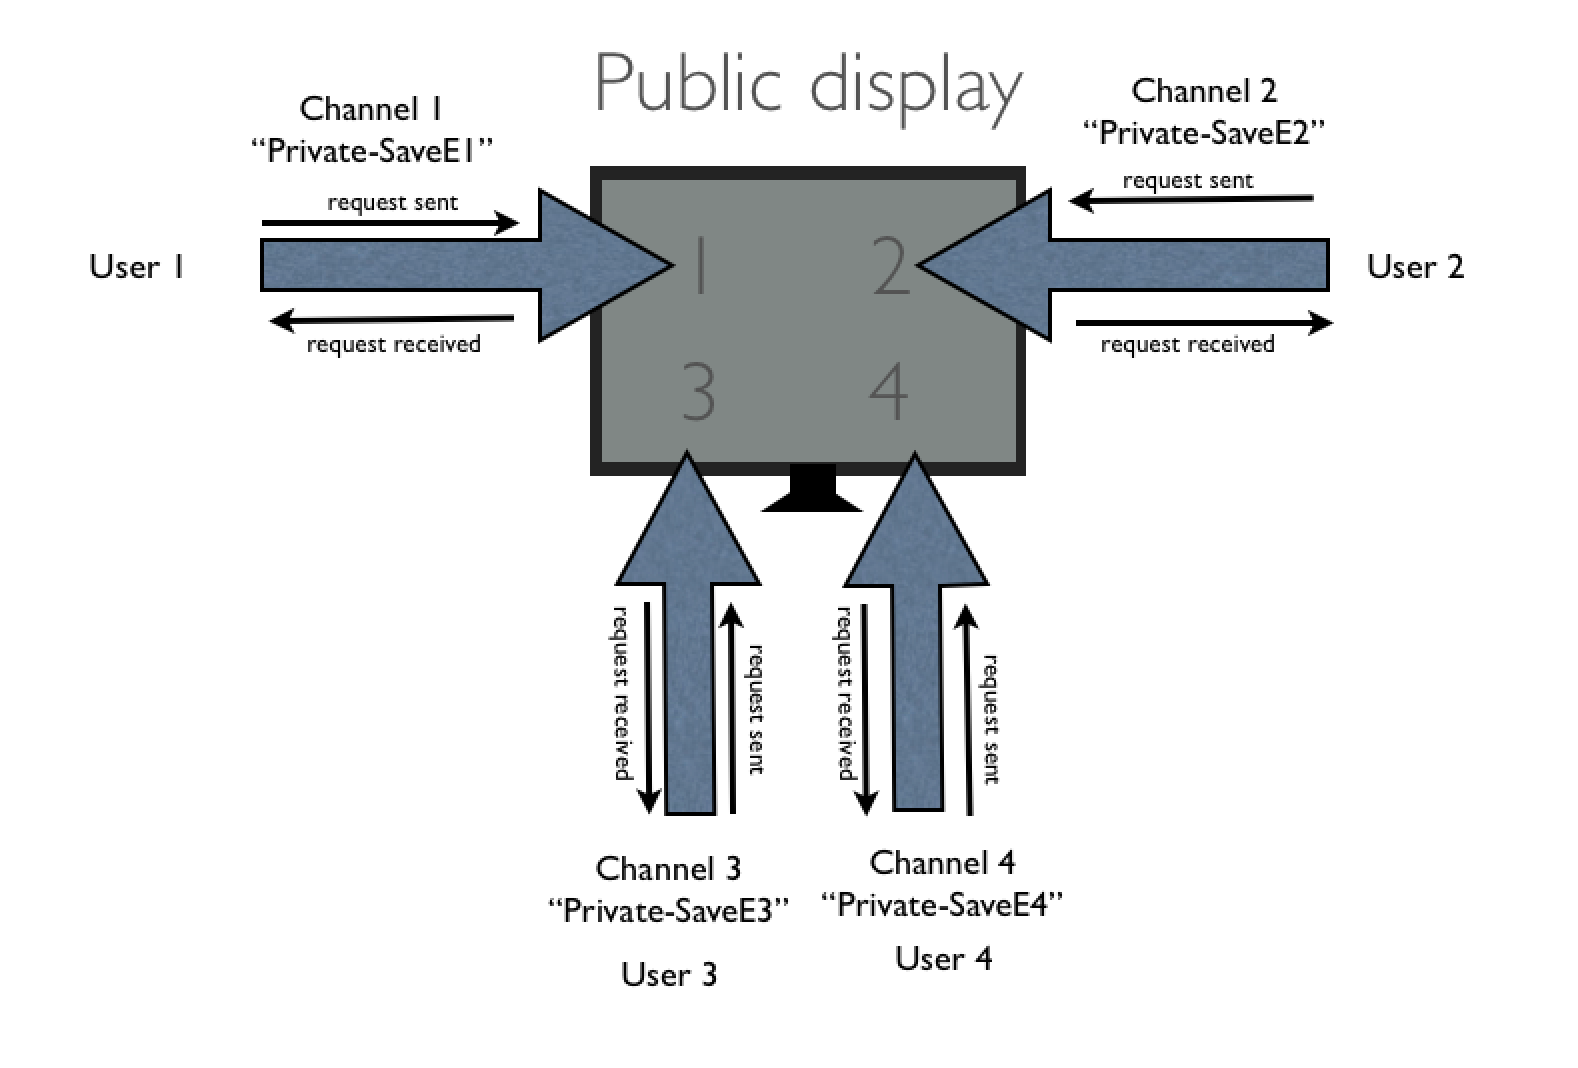
\includegraphics[width=1\textwidth]{ChannelsAndConnections.png}
\caption{This figure showing the connections and the channels and how every user connects via his own channel.}
\label{fig:ChannelsAndConnections}
\end{figure}


\section{Multi-user setup}
\label{sec:Multi-userSetup}
The multi-user setup was one of the challenging part in the project because normally when a web application is opened in a window it will have a session for the user opening that window but to have a number of users doing some actions in the same window here the problem occurs because each user is supposed to have one session id which is stored by the browser window but when multiple-users start to navigate in one window the sessions replace each other, as a result the requests origin or the user who made that request will not be known.
The problem was handled by passing the user id which is a unique key which identify a user to every page he visits once the user is logged in and neglecting the session id so doing this for all the users on the screen solves the problem of the sessions replacing each other and making sure to know where does this request comes from or from which user to avoid colliding of requests.

\newline \noindent The organising of the users on the display and the process of registering a user on the display in order to start interacting with it was done by implementing a simple algorithm it's goal is to organise the order of the users and their slots on the screen and to let the users interact on their specified slots and by saving the number of users currently on the display in a local storage variable by the browser.

\newline \noindent As you can see the following figure~\ref{fig:SlotNumbersAndStatus} 

\begin{figure}[H]
\centring
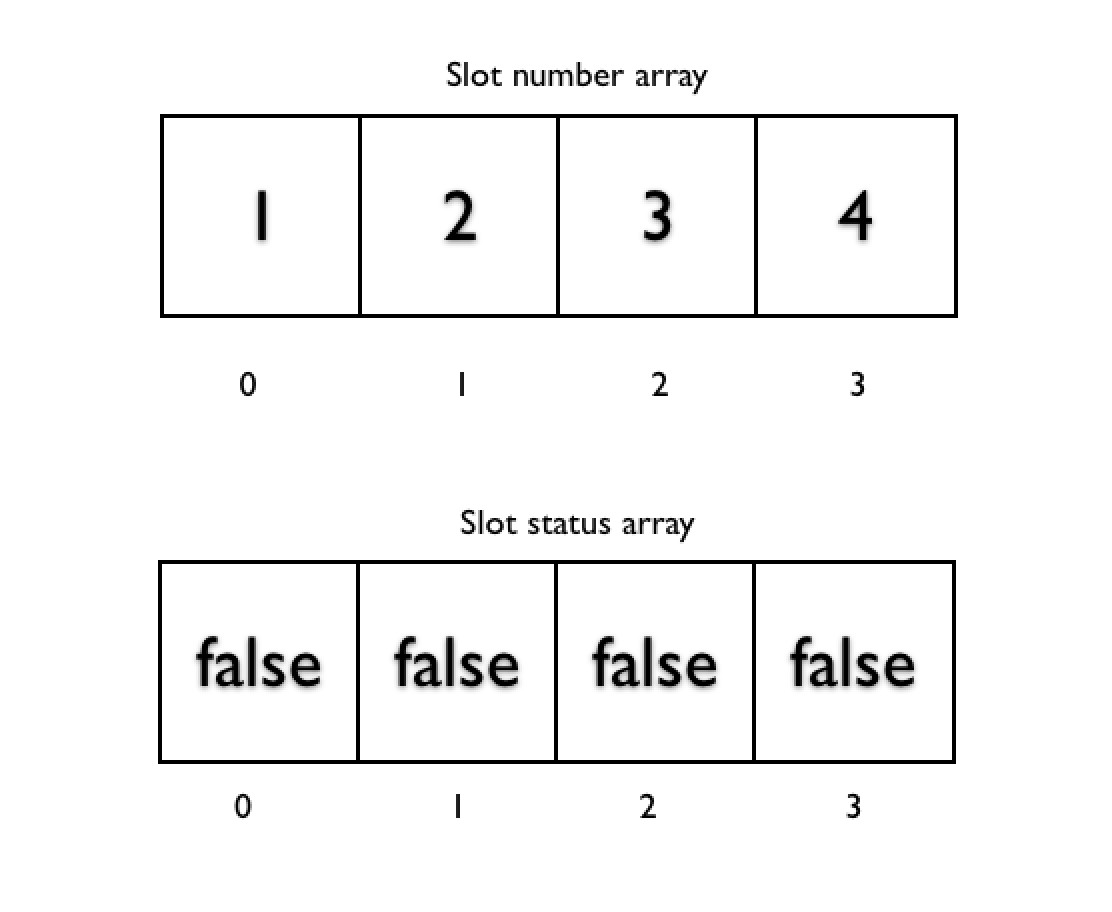
\includegraphics[width=1\textwidth]{SlotNumbersAndStatus.png}
\caption{The figure shows the array of slot numbers on the display.}
\label{fig:SlotNumbersAndStatus}
\end{figure}

\newline \noindent represents the array of screen slots numbers from 1 to 4 when a user press the connect button the mobile sends a signal via a general channel to the server which then loops on the slot status array in figure~\ref{fig:SlotNumbersAndStatus}.

%\begin{figure}[H]
%\centring
%\includegraphics[width=1\textwidth]{BooleanStatusArray.png}
%\caption{The figure shows an array of the status of each slot on the screen}
%\label{fig:BooleanStatusArray}
%\end{figure}

\newline \noindent And when it finds a free slot which means false it overrides the false value with a true one and take it's index to get the corresponding index in the slot numbers array in figure~\ref{fig:SlotNumbersAndStatus} then it sends the slot number which will be assigned to this user to the mobile device and connect to the channel of this number and display the content on the specified slot then it increment a local storage variable stored by the browser which keep track of the number of users on the display. For example imagine this situation :
currently the public display has 3 users logged-in and another user wants to connect so as you can see in figure~\ref{fig:Example1} the Boolean array which represents the current busy slots of the screen indicates that slot 1,2 and 3 are taken.

\begin{figure}[H]
\centring
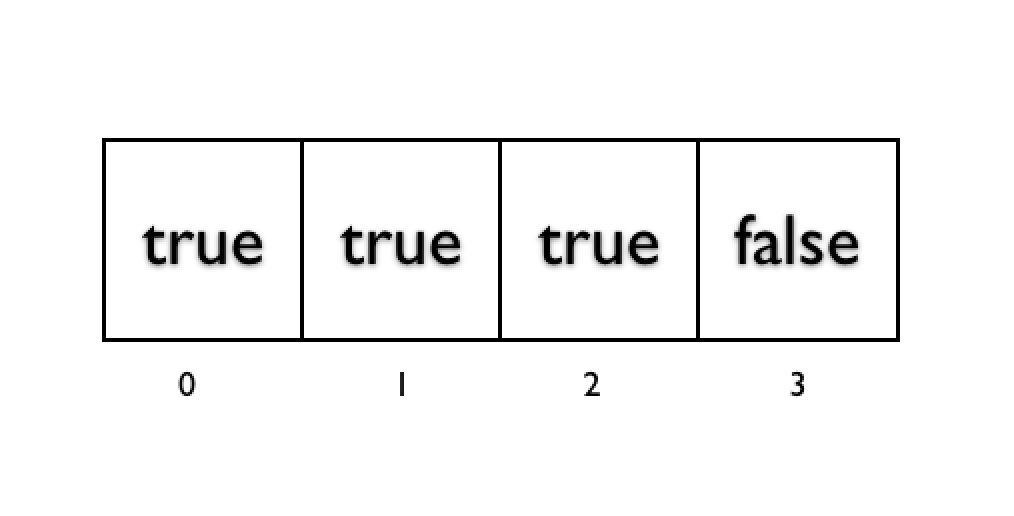
\includegraphics[width=0.75\textwidth]{Example1.png}
\caption{The figure shows an example of users available in slot 1,2 and 3 initially.}
\label{fig:Example1}
\end{figure}

\newline \noindent So once the user press connect what the system does is the following :

\begin{figure}[H]
\centring
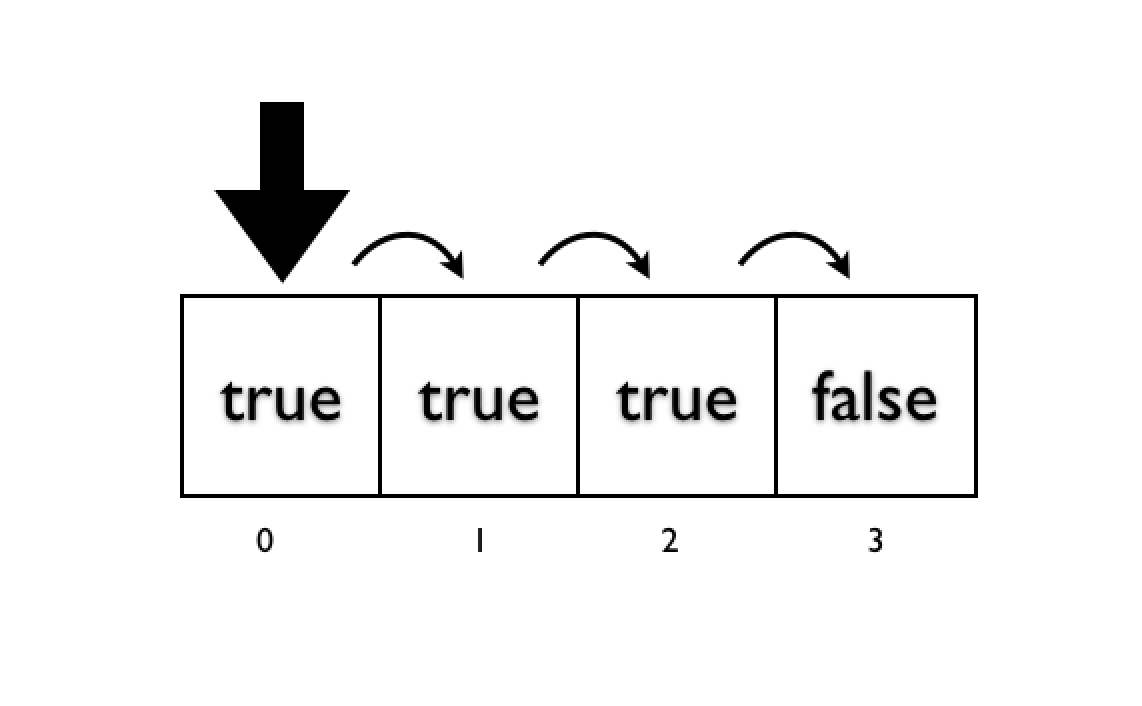
\includegraphics[width=0.75\textwidth]{Example2.png}
\caption{The system in the figure iterates on the array to find an empty slot or a false value in this case.}
\label{fig:Example2}
\end{figure}

\newline \noindent The system begin to loop on the array that contains the status of each slot on the screen until it find a cell in the array in which the cell is "false" which means at this index in the Slot number array the slot is free then the system stops and replace the status with true instead of false then sends this number to the mobile in order to connect on the channel of that slot to be able to interact so here is a figure when the algorithm executed.

\begin{figure}[H]
\centring
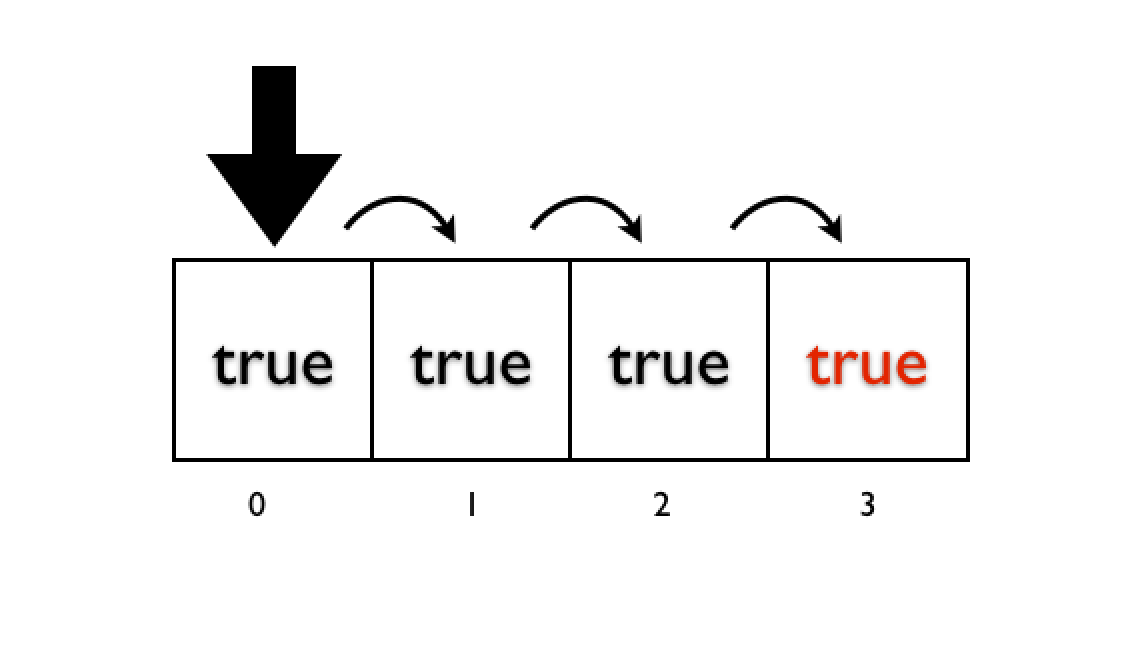
\includegraphics[width=0.75\textwidth]{Example3.png}
\caption{The figure shows that the system found an empty slot (false value) and will replace it with a true value to indicate that it is busy.}
\label{fig:Example3}
\end{figure}

\newline \noindent Then it sends the corresponding number in the slot numbers array which is 4 in this case to the mobile to be able to connect to slot 4 via its channel so as it appears in figure~\ref{fig:Example4} the number is then sent to the mobile and concatenated to the default channel name which is "Private-SaveE" as mentioned in the previous section. And by that it prevents any conflicts between users and let the system distinguish between user requests.

\begin{figure}[H]
\centring
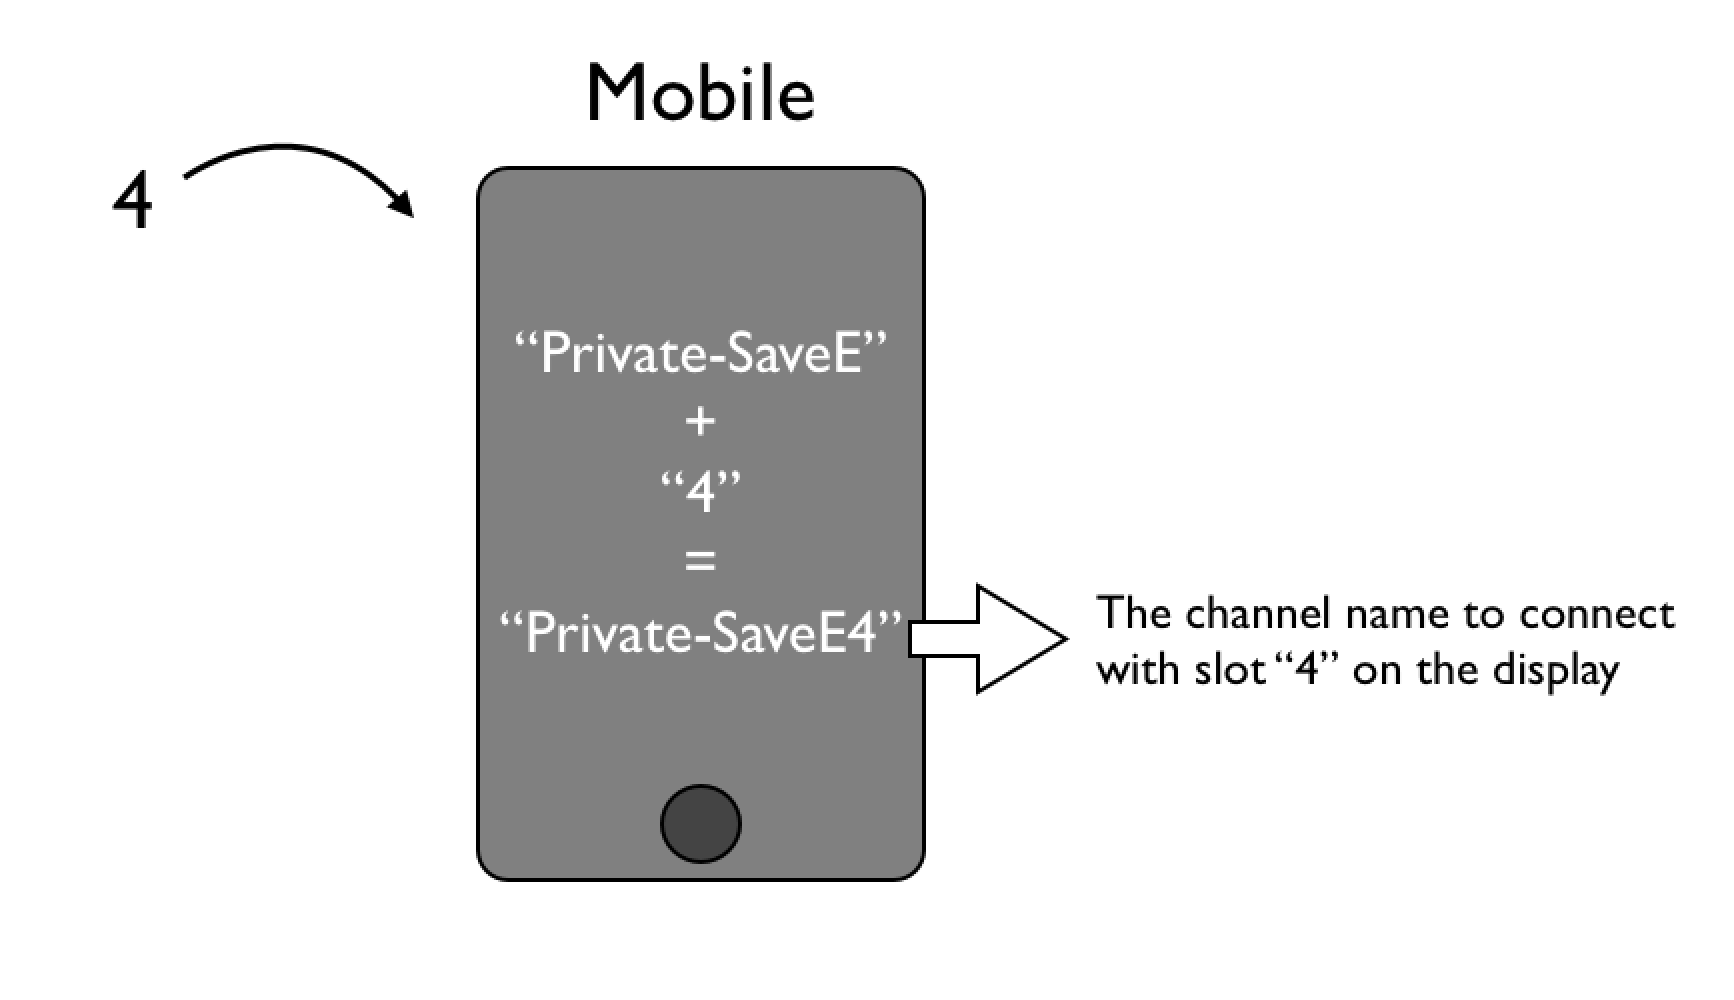
\includegraphics[width=0.75\textwidth]{Example4.png}
\caption{The figure shows when the number of slot is sent to the mobile then the mobile concatenate that number with the default channel name to connect to the corresponding channel.}
\label{fig:Example4}
\end{figure}

\section{Synchronization}
\label{sec:Synchronization}
Synchronization of the displays was done by also using the connections as mentioned in the Connections section \ref{sec:Connection} so the system once the user pressed any button on his mobile to navigate the system on the display the mobile pops-up the loading widget which tells the user what is the server trying to do in that moment so while the request reach the server, the server sends to the display what to show then an event is triggered on the channel which the user is connected to with a loading complete header which indicates that the request has successfully executed and the loading widget is removed from the user mobile screen and the page is changed to match the display contents. And here is an example to illustrate more :

\begin{figure}[H]
\centring
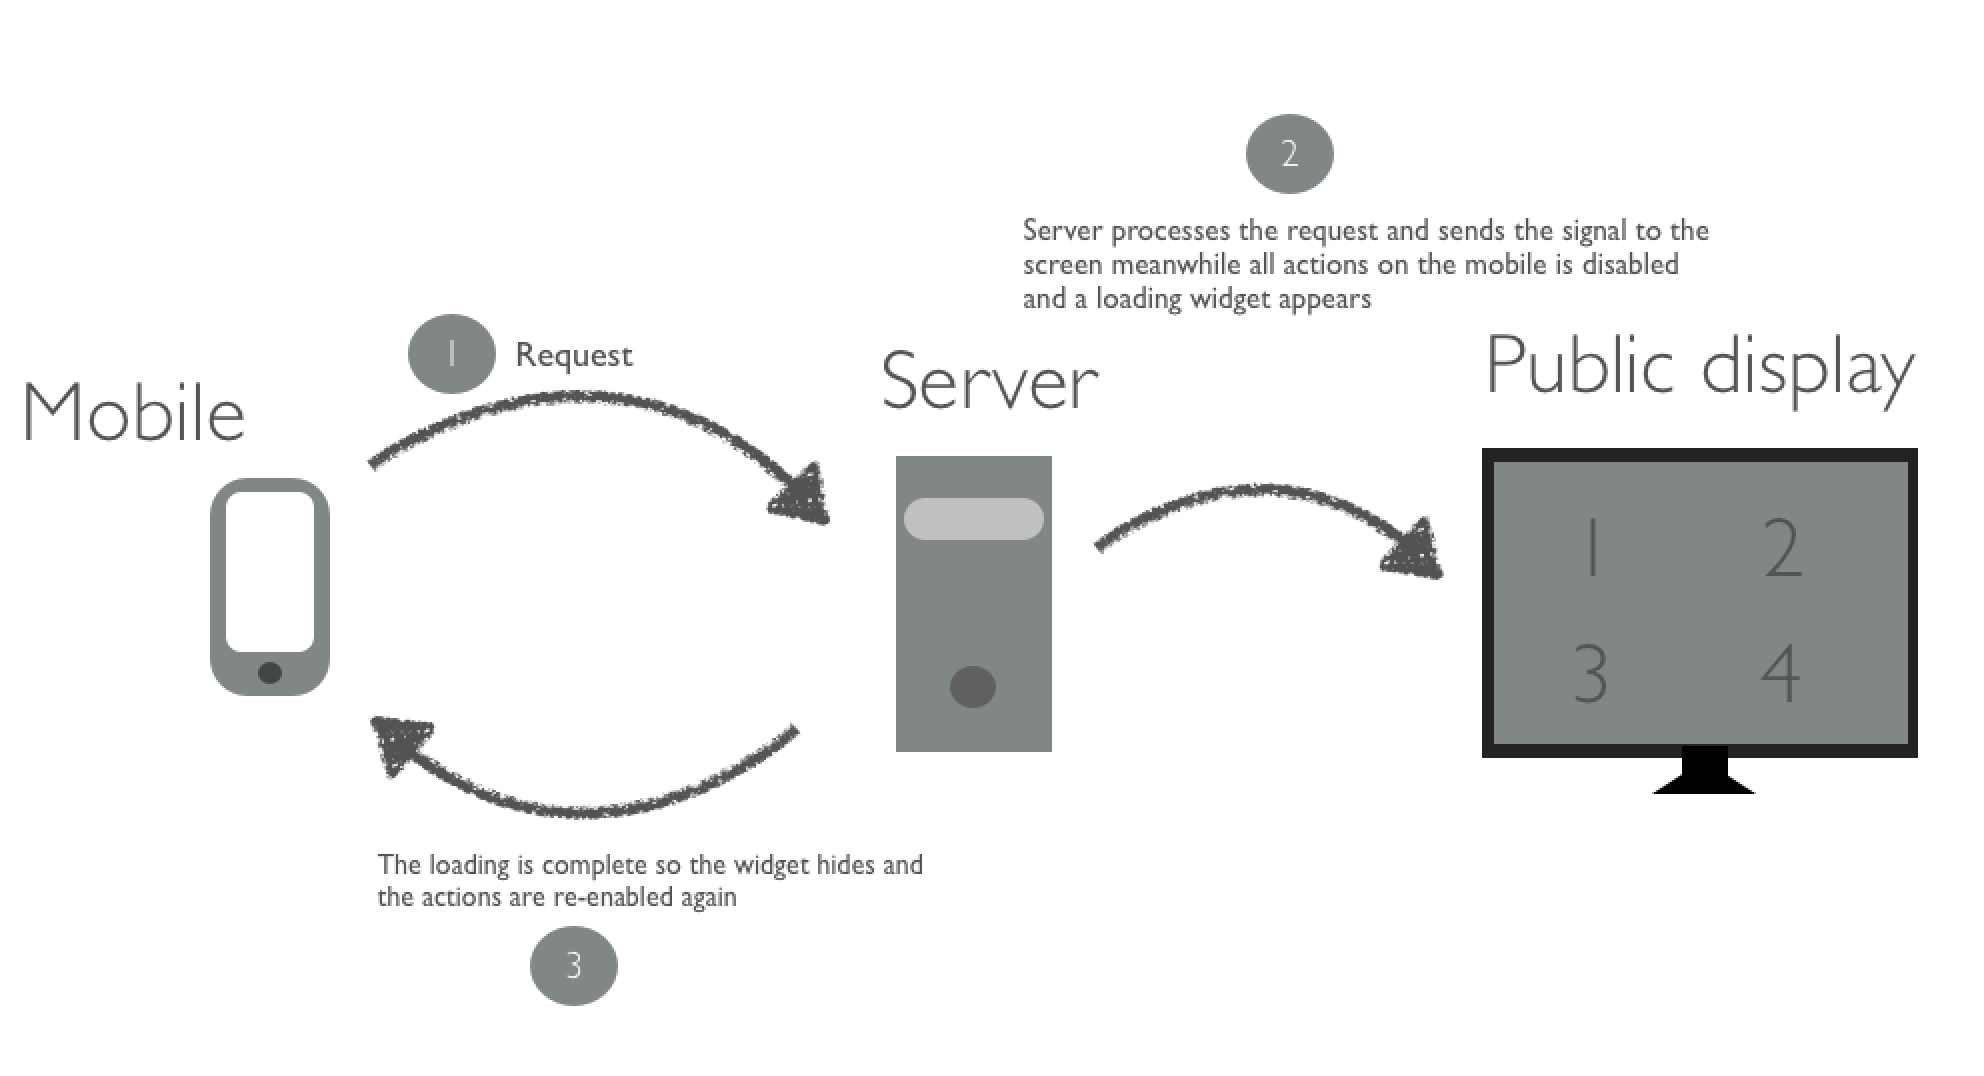
\includegraphics[width=1\textwidth]{Example7.png}
\caption{This figure illustrates the synchronization process.}
\label{fig:Example7}
\end{figure}

\section{Tip Generator}
\label{sec:TipGenerator}
The tip generator was implemented to help people change their daily lives action slightly a bit in order to save much more energy so for example when cooking if the pot is not covered then definitely there is a large amount of energy lost and you need to consume more energy in order to compensate for the energy you lost when removing the pot's cover and letting heat escape. So from here came the motivation to implement the tip generator to help people to change these very small actions or attitudes towards certain situations but saves loads of energy. As you can see in figure~\ref{fig:Example10} the tip generator generates tips organised according to its topic.

\begin{figure}[H]
\centring
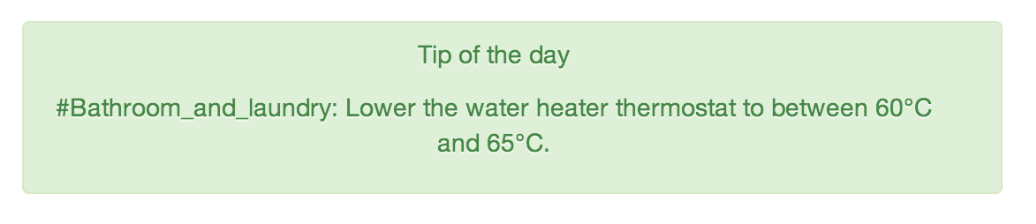
\includegraphics[width=1\textwidth]{Example10.png}
\caption{This figure the kind of tips generated by the tip generator.}
\label{fig:Example10}
\end{figure}

\section{Responsiveness And Interaction}
\label{sec:ResponsivenessAndInteraction}
One of the important milestones in the project were the responsiveness and the interactions since the application is a multi-user application so multiple user interface profiles had to be made in order to cover all the possible situations and combinations that might happen between users so for example when a user is on the display alone the user takes the whole screen alone to display his data but when 2 users are on the display the display in  splitter between them and both user interfaces for each user have to be changed in order to match the new dimensions and space that each user have on the display. So for more understanding please refer to this figure~\ref{fig:Example5} this is a situation when 1 user is navigating the display alone:

\begin{figure}[H]
\centring
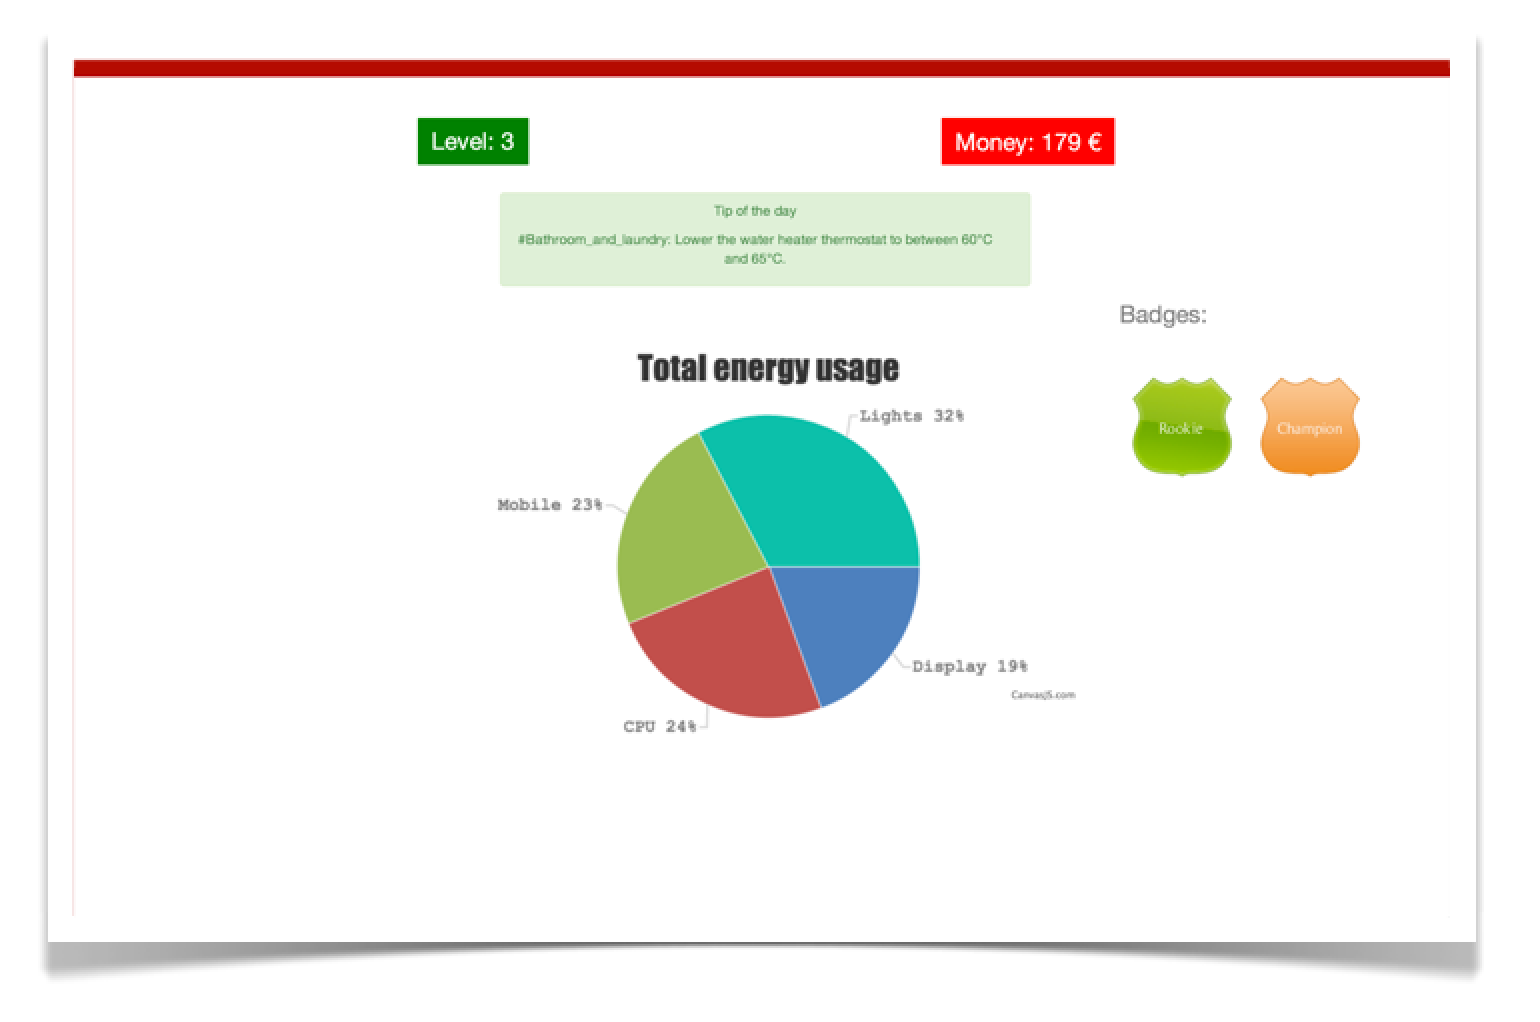
\includegraphics[width=0.85\textwidth]{Example5.png}
\caption{The figure shows only 1 user navigating the display.}
\label{fig:Example5}
\end{figure}

\newline \noindent Then if another user wants to log-in and navigates, the user interface of both users change according to the number of users which is stored by the browser in the local storage as mentioned in the connection section \ref{sec:Connection} and here is a figure to illustrate more:

\begin{figure}[H]
\centring
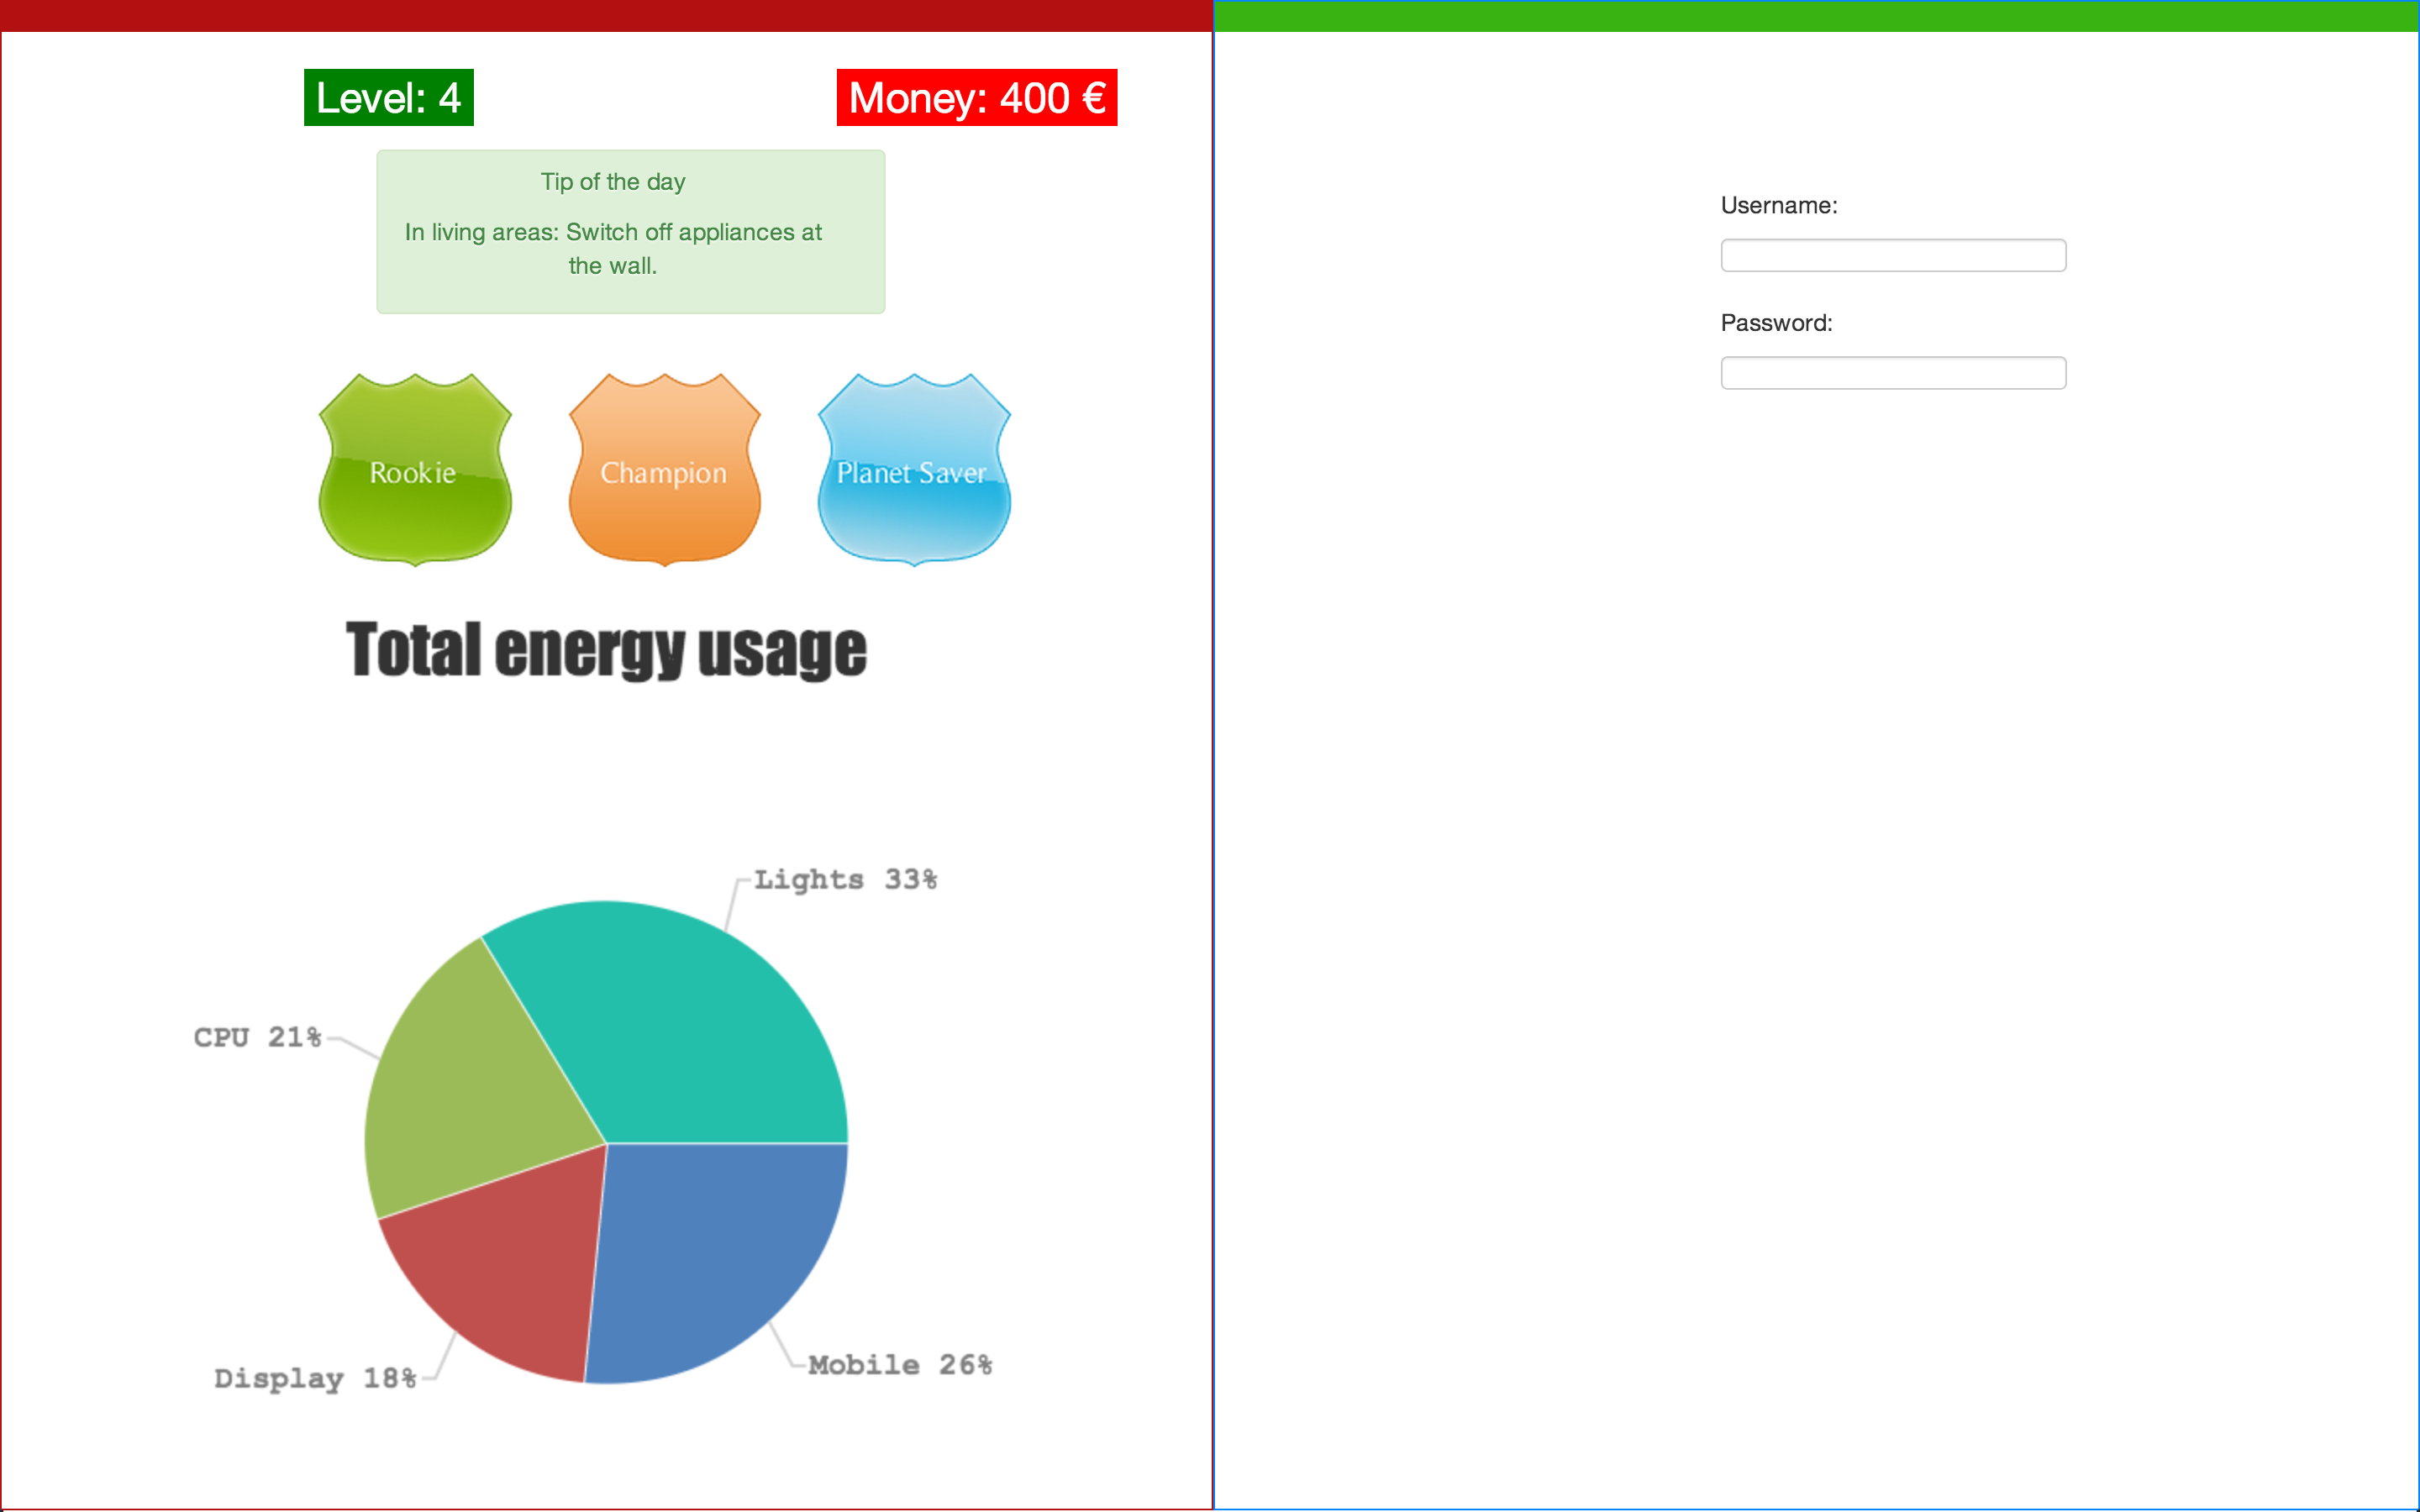
\includegraphics[width=0.85\textwidth]{Example6.png}
\caption{The figure shows the screen when another user connected.}
\label{fig:Example6}
\end{figure}

\newline \noindent This was made by implementing css classes for each element on the screen for each possible scenario for example when a user navigates on the display alone he is taking the whole screen alone and all the elements are given the css for that situation but then when another user signs in he trigger a function which then knows the page that each user is currently at and begin to change the css of each of the elements to the new situation so the css is all checked and changed when a user connects to the display and already there are other users. Also when a user navigates from one page to another, the same function is called but to only correct the css of any change happened and to maintain the correct user interface for all the users.


\section{User Data}
\label{sec:UserData}
User data which is simply represented as charts in the project and letting the user know their energy consumption was one of the objectives to increase energy awareness and to help users save energy so user data had to be made in order to illustrate to the user his consumption also helps in 2 points:
\newline the first point: user data helps the user to know their detailed energy consumption and as a result the user can know where does the problem come from or from which device he consumes energy the most.
\newline the second point: users may take advantage of the multi-user setup and use the system to compare each other's data in order to motivate both of them to save energy as that can give them rewards as we will see in the game mechanics section\ref{sec:GameMechanics}.

\section{User Privacy}
\label{sec:UserPrivacy}
Privacy was one of the important aspects of the project since the project was not about creating an application to motivate people to save energy and increase their energy awareness only , but also a robust and trusted system, so privacy had to be implemented in the project in order to let the user feel safe at any time he doesn't want anyone to check his detailed energy consumption he just can hide his data from people and view it on his mobile screen instantaneously. So 2 privacy modes were created the high privacy mode which tells the system to hide the data from the public display and send the data to the mobile so the user only see his data on his mobile once he choose that option and the low privacy mode which is the normal mode , the data is kept at the display available for all users to see normally.
\\
\newline \noindent But while trying to implement privacy there were certain constraints:
\newline \noindent first the size limit of pusher service used for the connection between the public display and the mobile was only 10KB so sending the whole page to the mobile from the screen was not an option.
\newline \noindent second the css and user interface of the page on the screen was displayed using twitter bootstrap as mentioned in section \ref{sec:TechnologiesUsed} and on the mobile Jquery mobile was used , so 2 different technologies used as the interface for each the display and the mobile, as a result the data couldn't be sent directly to the mobile since the styles will replace each other.
\\
\newline \noindent The 2 problems were solved by just sending the crucial information which was the user data in this case because there is no point in hiding the level or the money you have because it already appears on the leader board and they are made to let people compete with each other not hide it from each other so the charts engine used were put on the mobile and the data of the charts was the only part sent so by that the first problem which was the size was solved also the second one was solved because nothing is required to be sent with the data and then the mobile gives the data to the charts engine on the mobile to render it and generate the charts on the mobile once the user chooses the high privacy option.

\begin{figure}[H]
\centring
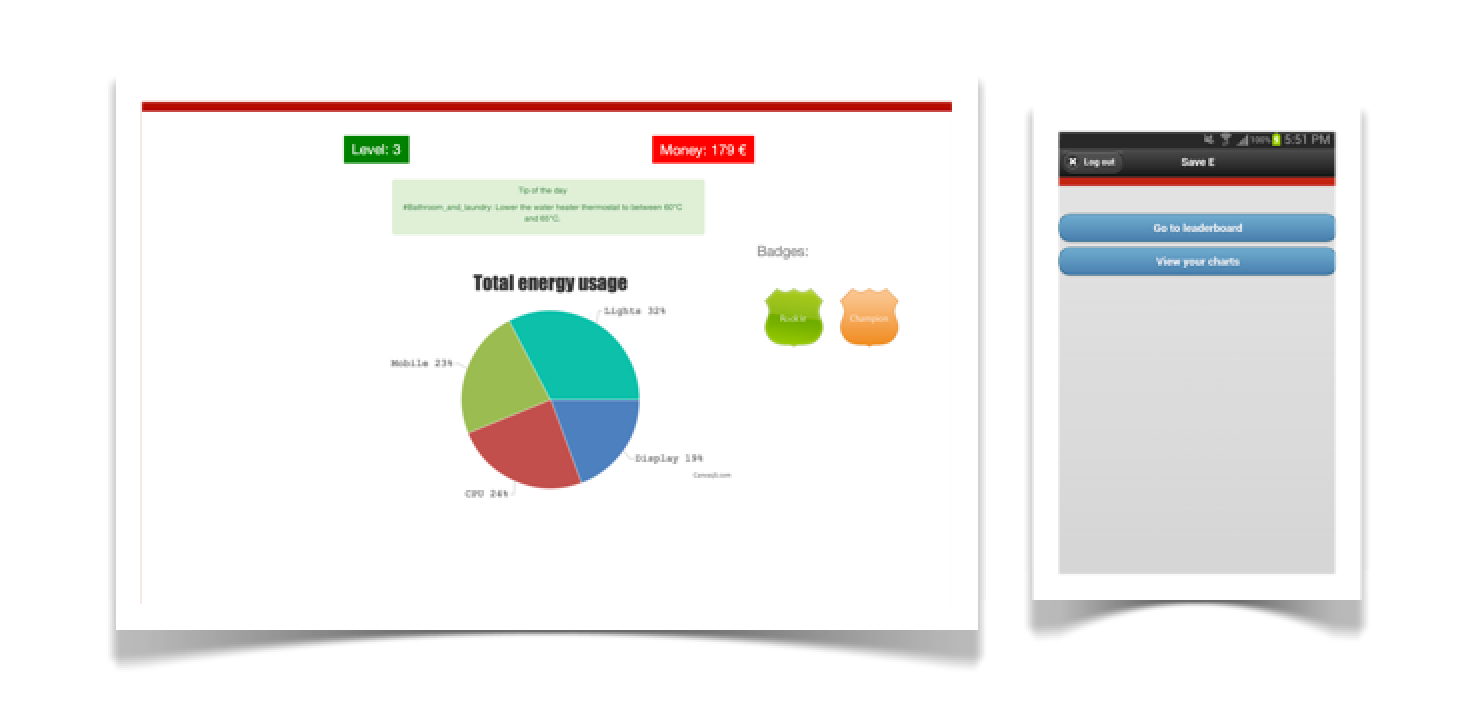
\includegraphics[width=1\textwidth]{Example8.png}
\caption{This figure shows the screen and the mobile in low privacy profile settings.}
\label{fig:Example8}
\end{figure}

\begin{figure}[H]
\centring
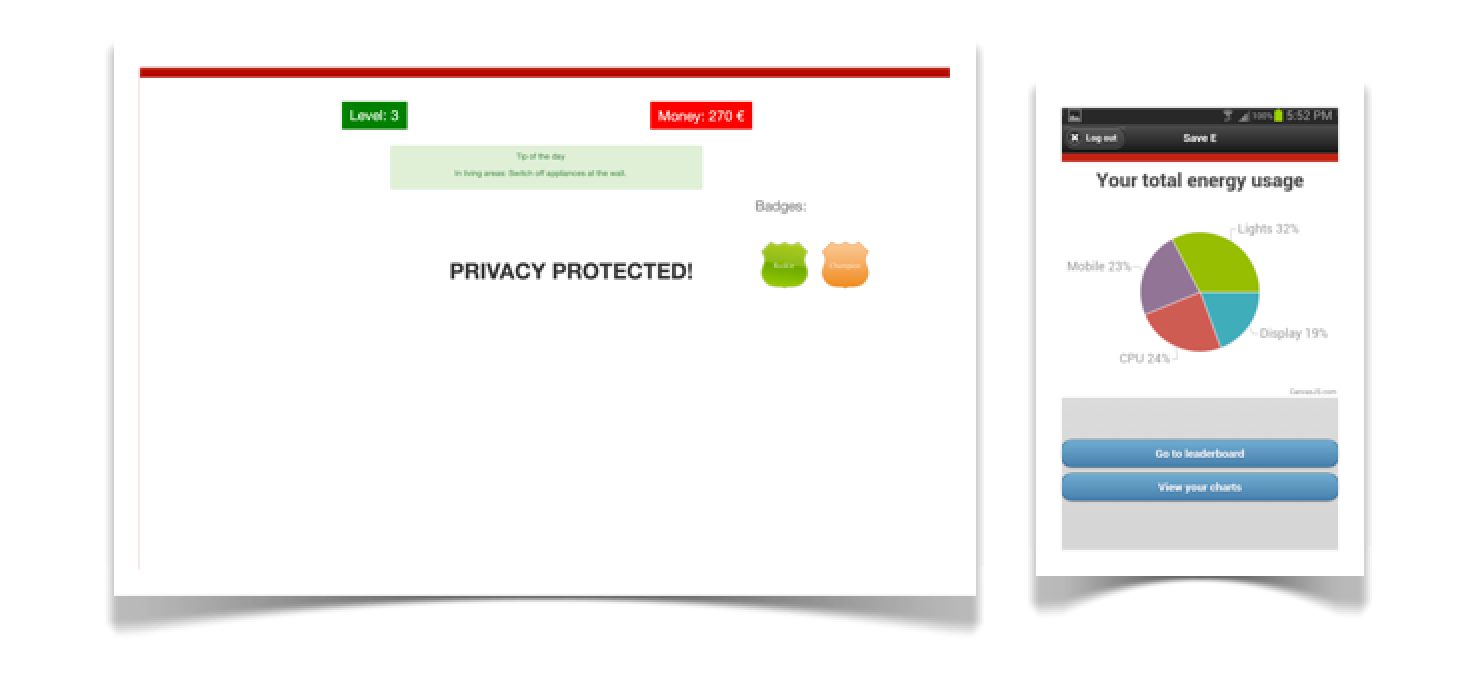
\includegraphics[width=1\textwidth]{Example9.png}
\caption{This figure shows the screen and the mobile when the user chooses high privacy profile settings.}
\label{fig:Example9}
\end{figure}

\section{Game Mechanics}
\label{sec:GameMechanics}
Gamification or applying game mechanics is now widely used in many applications because it enhance the user experience with the application and involves more fun but in the same time it motivates users to challenge and compete against each other in order to be from the top 3 or the top 10 players so this concept was used in the project to bring more interaction between the users and increase their motivation to compete against each other to save energy and gain badges and virtual money to be able to make their way up the leader board as it will be explained later in this section.

\newline \noindent So simply the game mechanics of the system consists of:
\\
\newline \noindent 1- Levels: level is an indication about your total consumption also used by the leader board as the sorting key.
\newline \noindent 2- Badges: a badge is gained when you cross a certain amount of money and as long as you are saving more money you gain more badges.
\newline \noindent 3- Virtual Money: initially users have money then when the costs of their usages is calculated and deducted they loose them.
\newline \noindent 4- Leader board: the leader board is the place where you can see all the users and their levels,badges,money and ranks.
\\
\newline \noindent So simply users at first have a certain amount of money by default then when they start measuring their energy consumption day by day the cost is calculated and deducted from the money they have so the more you consume energy the less the money you have and vice versa. Also when the system detects that the data is for a new month the system adds new money to the users so when the users save more energy and pay less, their money increase and when they reach a certain amount of money which is decided by the system, they gain badges which leads to a level up and improving their ranks on the leader board.

%******************************************************************************
% CONCLUSION
%******************************************************************************

\chapter{Conclusion}
\label{chap:Conclusion}

%******************************************************************************
% RESULTS AND FUTURE WORK
%******************************************************************************

\chapter{Results And Future Work}
\label{chap:ResultsAndFutureWork}

\section{Experiment}
\label{sec:Experiment}
A study had to be made in order to test the system in many aspects some of them were usability,trust,complexity and motivation to save energy so the study was performed with 10 participants the nationalities were Germans, Indians, Egyptians. 3 of the Users were females while the other 7 where males. The study was done by giving the users an introduction about the application and then leaving them with a list of tasks to try to accomplish them, the study focused more on the usability,easiness and interaction of the system more than of the motivation the users got after using the system to save energy.



%******************************************************************************
% BIBLIOGRAPHY
%******************************************************************************



%******************************************************************************
% BIBLIOGRAPHY
%******************************************************************************
\bibliographystyle{plain}
{\small\bibliography{master}}

%******************************************************************************
% APPENDIX
%******************************************************************************
\appendix
\appendixpage*
\chapter{FirstAppendix}
\label{app:FirstAppendix}
%This is the place where the appendices are supposed to be. Appendices are everything that would just blow up your thesis but are still of some interest for a reader that wants to get a deeper grasp on the details of your work.


%******************************************************************************
% BACK MATTER
%******************************************************************************
\backmatter

%******************************************************************************
% LIST OF SYMBOLS
%******************************************************************************
%\normalfont
%\clearpage
%\chapter[List of Symbols and Abbreviations]{List of Symbols and Abbreviations}
%\begin{center}
%\small
%\begin{longtable}{lp{3.0in}c}
%\toprule
%\multicolumn{1}{c}{Abbreviation} & \multicolumn{1}{c}{Description}\\ \midrule\addlinespace[2pt] \endhead
%\bottomrule\endfoot
%XML & E\textbf{X}tensible \textbf{M}arkup \textbf{L}anguage \\
%XSD & \textbf{X}ML-\textbf{S}chema-\textbf{D}efinition \\
%SFXML & \textbf{S}cene\textbf{F}low E\textbf{X}tensible \textbf{M}arkup \textbf{L}anguage \\
%SFTXL & \textbf{S}cene\textbf{F}low \textbf{T}extual E\textbf{X}pression \textbf{L}anguage \\
%SCXML & \textbf{S}tate\textbf{C}hart E\textbf{X}tensible \textbf{M}arkup \textbf{L}anguage \\
%DOM & \textbf{D}ocument \textbf{O}bject \textbf{M}odel \\
%LR & \textbf{L}eft to \textbf{R}ightmost derivation \\
%LALR & \textbf{L}ook\textbf{A}head LR\\
%NPC & \textbf{N}on-\textbf{P}erson-\textbf{C}haracter\\
%ABL & \textbf{A} \textbf{B}ehavior \textbf{L}anguage\\
%\end{longtable}
%\end{center}

%******************************************************************************
% LIST OF FIGURES
%******************************************************************************
\normalfont
\clearpage
\listoffigures

%******************************************************************************
% LIST OF TABLES
%******************************************************************************
\normalfont
\clearpage
\listoftables

%******************************************************************************
% LIST OF ALGORITHMS
%******************************************************************************
%\normalfont
\clearpage
\listofalgorithms

%******************************************************************************
% END DOCUMENT
%******************************************************************************
\end{document}
